% Copyright (c) 2013 Benky
% This program is made available under the terms of the MIT License.
\documentclass{article}
\usepackage{tikz}
\usepackage{mathpazo}
\usepackage[top=20mm,left=20mm,right=0mm,bottom=0mm,a1paper]{geometry}
\usepackage{verbatim}

\begin{document}

% 1MoA = ((2*Pi*300)/(360*60))*100
\newcommand{\OneMOA}{145.37037037037038mm}


% Red diamond with cross
\newcommand\benkysCross{
  \draw[fill=white, color=white] (0cm,0cm) rectangle (10cm,-10cm);
  \draw[line width=2mm, fill=black] (0cm, 0cm) circle [radius=17mm];
  \draw[line width=2mm] (0cm, 0cm) circle [radius=64mm]; % << poor man's spacing :-/

  \draw[line width=4mm, color=white] (-10mm, -10mm) -- (10mm, 10mm);
  \draw[line width=4mm, color=white] (-10mm, 10mm) -- (10mm, -10mm);  
}

\begin{tikzpicture}
  \begin{scope}[shift={(5,5)}]
    \benkysCross
  \end{scope}
  \begin{scope}[shift={(25,5)}]
    \benkysCross
  \end{scope}
  \begin{scope}[shift={(45,5)}]
    \benkysCross
  \end{scope}
\end{tikzpicture}

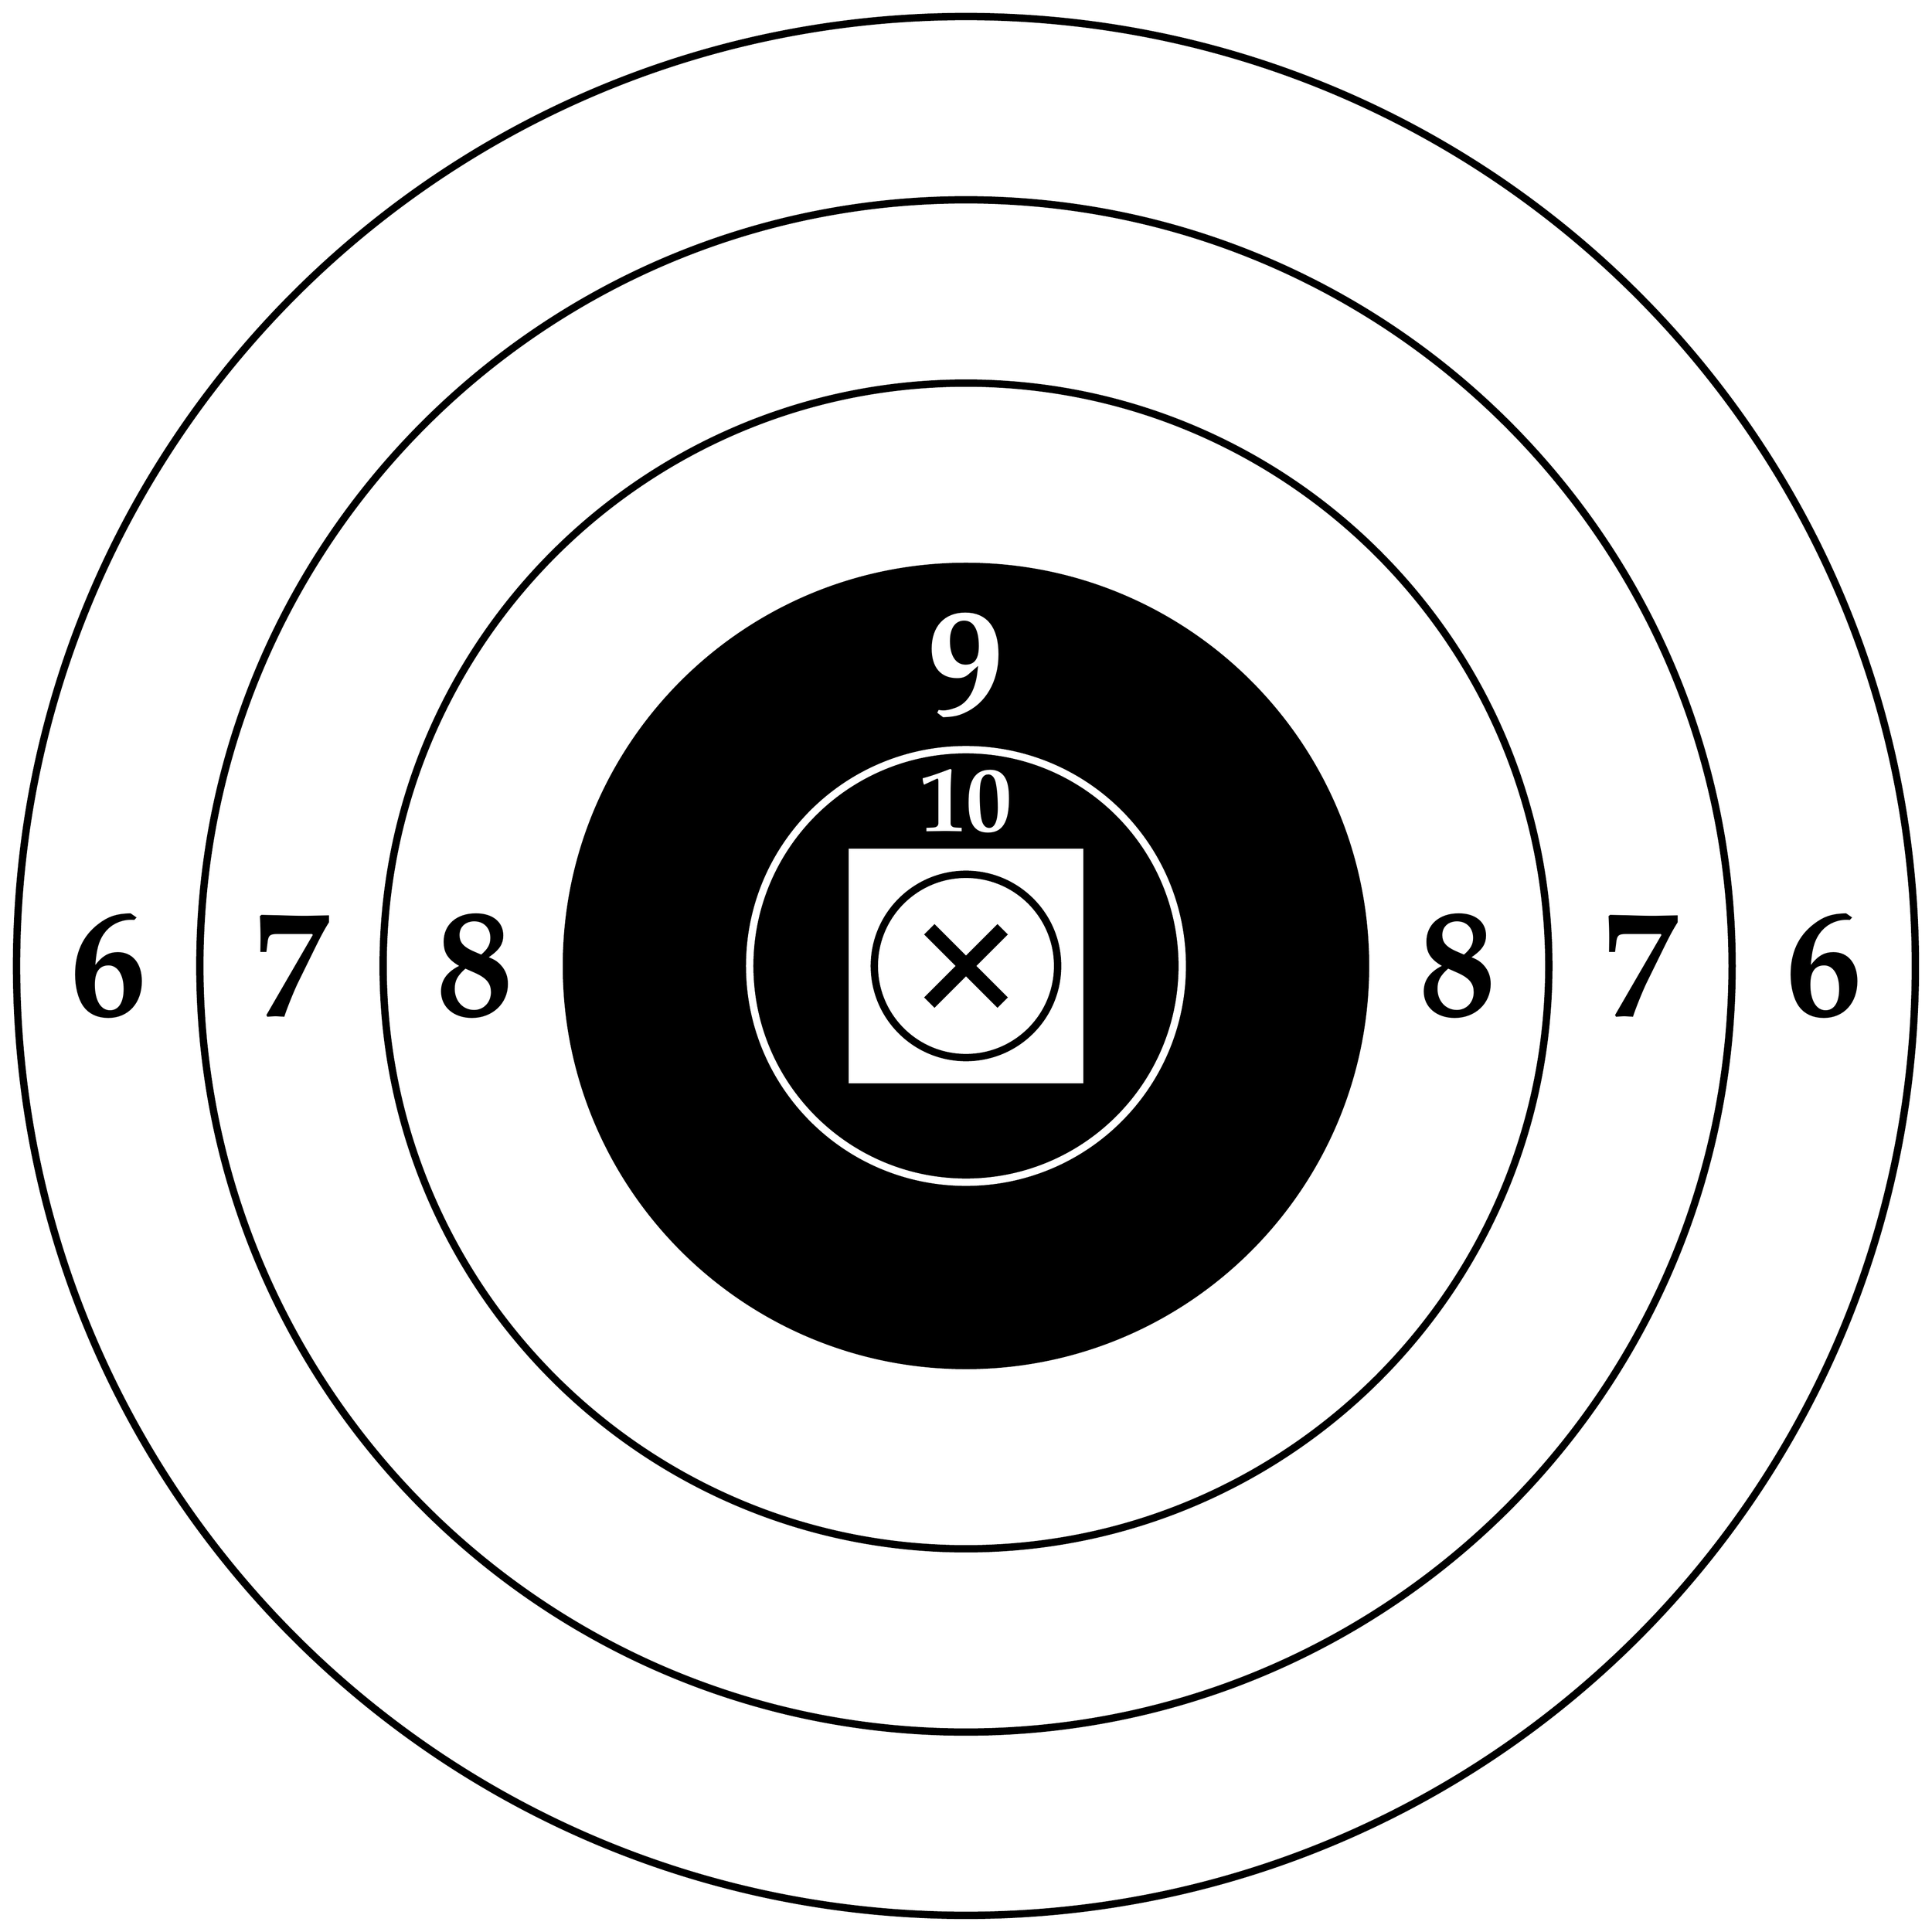
\begin{tikzpicture}
  \begin{scope}[shift={(210mm,300mm)}]
    \draw[line width=2mm, fill=black] (0cm, 0cm) circle (218mm/2); % 9
    \draw[line width=2mm, color=white, fill=black] (0cm, 0cm) circle (118mm/2); % 10
    \draw[line width=2mm, color=black, fill=white] (-33mm, -33mm) rectangle (33mm, 33mm); % box
    \draw[line width=2mm, color=black, fill=white] (0cm, 0cm) circle (50mm/2); % X    

    \draw[line width=4mm] (-10mm, -10mm) -- (10mm, 10mm);
    \draw[line width=4mm] (-10mm, 10mm) -- (10mm, -10mm);
    
    \node[scale=6.0, color=white] at (0mm, 45mm) {\large \textbf{10}};
    \node[scale=10.0, color=white] at (0mm, 82mm) {\large \textbf{9}};
    
    \draw[line width=2mm] (0cm, 0cm) circle (318mm/2);
    \draw[line width=2mm] (0cm, 0cm) circle (418mm/2);
    \draw[line width=2mm] (0cm, 0cm) circle (518mm/2);

    \node[scale=10.0, color=black] at (134mm, 0mm) {\large \textbf{8}};
    \node[scale=10.0, color=black] at (184mm, 0mm) {\large \textbf{7}};
    \node[scale=10.0, color=black] at (234mm, 0mm) {\large \textbf{6}};        

    \node[scale=10.0, color=black] at (-134mm, 0mm) {\large \textbf{8}};
    \node[scale=10.0, color=black] at (-184mm, 0mm) {\large \textbf{7}};
    \node[scale=10.0, color=black] at (-234mm, 0mm) {\large \textbf{6}};        
\end{scope}
\end{tikzpicture}


\end{document}
